% Options for packages loaded elsewhere
\PassOptionsToPackage{unicode}{hyperref}
\PassOptionsToPackage{hyphens}{url}
\documentclass[
]{article}
\usepackage{xcolor}
\usepackage[margin=1in]{geometry}
\usepackage{amsmath,amssymb}
\setcounter{secnumdepth}{-\maxdimen} % remove section numbering
\usepackage{iftex}
\ifPDFTeX
  \usepackage[T1]{fontenc}
  \usepackage[utf8]{inputenc}
  \usepackage{textcomp} % provide euro and other symbols
\else % if luatex or xetex
  \usepackage{unicode-math} % this also loads fontspec
  \defaultfontfeatures{Scale=MatchLowercase}
  \defaultfontfeatures[\rmfamily]{Ligatures=TeX,Scale=1}
\fi
\usepackage{lmodern}
\ifPDFTeX\else
  % xetex/luatex font selection
\fi
% Use upquote if available, for straight quotes in verbatim environments
\IfFileExists{upquote.sty}{\usepackage{upquote}}{}
\IfFileExists{microtype.sty}{% use microtype if available
  \usepackage[]{microtype}
  \UseMicrotypeSet[protrusion]{basicmath} % disable protrusion for tt fonts
}{}
\makeatletter
\@ifundefined{KOMAClassName}{% if non-KOMA class
  \IfFileExists{parskip.sty}{%
    \usepackage{parskip}
  }{% else
    \setlength{\parindent}{0pt}
    \setlength{\parskip}{6pt plus 2pt minus 1pt}}
}{% if KOMA class
  \KOMAoptions{parskip=half}}
\makeatother
\usepackage{color}
\usepackage{fancyvrb}
\newcommand{\VerbBar}{|}
\newcommand{\VERB}{\Verb[commandchars=\\\{\}]}
\DefineVerbatimEnvironment{Highlighting}{Verbatim}{commandchars=\\\{\}}
% Add ',fontsize=\small' for more characters per line
\usepackage{framed}
\definecolor{shadecolor}{RGB}{248,248,248}
\newenvironment{Shaded}{\begin{snugshade}}{\end{snugshade}}
\newcommand{\AlertTok}[1]{\textcolor[rgb]{0.94,0.16,0.16}{#1}}
\newcommand{\AnnotationTok}[1]{\textcolor[rgb]{0.56,0.35,0.01}{\textbf{\textit{#1}}}}
\newcommand{\AttributeTok}[1]{\textcolor[rgb]{0.13,0.29,0.53}{#1}}
\newcommand{\BaseNTok}[1]{\textcolor[rgb]{0.00,0.00,0.81}{#1}}
\newcommand{\BuiltInTok}[1]{#1}
\newcommand{\CharTok}[1]{\textcolor[rgb]{0.31,0.60,0.02}{#1}}
\newcommand{\CommentTok}[1]{\textcolor[rgb]{0.56,0.35,0.01}{\textit{#1}}}
\newcommand{\CommentVarTok}[1]{\textcolor[rgb]{0.56,0.35,0.01}{\textbf{\textit{#1}}}}
\newcommand{\ConstantTok}[1]{\textcolor[rgb]{0.56,0.35,0.01}{#1}}
\newcommand{\ControlFlowTok}[1]{\textcolor[rgb]{0.13,0.29,0.53}{\textbf{#1}}}
\newcommand{\DataTypeTok}[1]{\textcolor[rgb]{0.13,0.29,0.53}{#1}}
\newcommand{\DecValTok}[1]{\textcolor[rgb]{0.00,0.00,0.81}{#1}}
\newcommand{\DocumentationTok}[1]{\textcolor[rgb]{0.56,0.35,0.01}{\textbf{\textit{#1}}}}
\newcommand{\ErrorTok}[1]{\textcolor[rgb]{0.64,0.00,0.00}{\textbf{#1}}}
\newcommand{\ExtensionTok}[1]{#1}
\newcommand{\FloatTok}[1]{\textcolor[rgb]{0.00,0.00,0.81}{#1}}
\newcommand{\FunctionTok}[1]{\textcolor[rgb]{0.13,0.29,0.53}{\textbf{#1}}}
\newcommand{\ImportTok}[1]{#1}
\newcommand{\InformationTok}[1]{\textcolor[rgb]{0.56,0.35,0.01}{\textbf{\textit{#1}}}}
\newcommand{\KeywordTok}[1]{\textcolor[rgb]{0.13,0.29,0.53}{\textbf{#1}}}
\newcommand{\NormalTok}[1]{#1}
\newcommand{\OperatorTok}[1]{\textcolor[rgb]{0.81,0.36,0.00}{\textbf{#1}}}
\newcommand{\OtherTok}[1]{\textcolor[rgb]{0.56,0.35,0.01}{#1}}
\newcommand{\PreprocessorTok}[1]{\textcolor[rgb]{0.56,0.35,0.01}{\textit{#1}}}
\newcommand{\RegionMarkerTok}[1]{#1}
\newcommand{\SpecialCharTok}[1]{\textcolor[rgb]{0.81,0.36,0.00}{\textbf{#1}}}
\newcommand{\SpecialStringTok}[1]{\textcolor[rgb]{0.31,0.60,0.02}{#1}}
\newcommand{\StringTok}[1]{\textcolor[rgb]{0.31,0.60,0.02}{#1}}
\newcommand{\VariableTok}[1]{\textcolor[rgb]{0.00,0.00,0.00}{#1}}
\newcommand{\VerbatimStringTok}[1]{\textcolor[rgb]{0.31,0.60,0.02}{#1}}
\newcommand{\WarningTok}[1]{\textcolor[rgb]{0.56,0.35,0.01}{\textbf{\textit{#1}}}}
\usepackage{longtable,booktabs,array}
\usepackage{calc} % for calculating minipage widths
% Correct order of tables after \paragraph or \subparagraph
\usepackage{etoolbox}
\makeatletter
\patchcmd\longtable{\par}{\if@noskipsec\mbox{}\fi\par}{}{}
\makeatother
% Allow footnotes in longtable head/foot
\IfFileExists{footnotehyper.sty}{\usepackage{footnotehyper}}{\usepackage{footnote}}
\makesavenoteenv{longtable}
\usepackage{graphicx}
\makeatletter
\newsavebox\pandoc@box
\newcommand*\pandocbounded[1]{% scales image to fit in text height/width
  \sbox\pandoc@box{#1}%
  \Gscale@div\@tempa{\textheight}{\dimexpr\ht\pandoc@box+\dp\pandoc@box\relax}%
  \Gscale@div\@tempb{\linewidth}{\wd\pandoc@box}%
  \ifdim\@tempb\p@<\@tempa\p@\let\@tempa\@tempb\fi% select the smaller of both
  \ifdim\@tempa\p@<\p@\scalebox{\@tempa}{\usebox\pandoc@box}%
  \else\usebox{\pandoc@box}%
  \fi%
}
% Set default figure placement to htbp
\def\fps@figure{htbp}
\makeatother
\setlength{\emergencystretch}{3em} % prevent overfull lines
\providecommand{\tightlist}{%
  \setlength{\itemsep}{0pt}\setlength{\parskip}{0pt}}
\usepackage{booktabs}
\usepackage{longtable}
\usepackage{array}
\usepackage{multirow}
\usepackage{wrapfig}
\usepackage{float}
\usepackage{colortbl}
\usepackage{pdflscape}
\usepackage{tabu}
\usepackage{threeparttable}
\usepackage{threeparttablex}
\usepackage[normalem]{ulem}
\usepackage{makecell}
\usepackage{xcolor}
\usepackage{bookmark}
\IfFileExists{xurl.sty}{\usepackage{xurl}}{} % add URL line breaks if available
\urlstyle{same}
\hypersetup{
  pdftitle={Midterm Project- R Code and Outputs},
  hidelinks,
  pdfcreator={LaTeX via pandoc}}

\title{Midterm Project- R Code and Outputs}
\author{}
\date{\vspace{-2.5em}}

\begin{document}
\maketitle

\subsection{Load in neccessary
packages}\label{load-in-neccessary-packages}

\begin{Shaded}
\begin{Highlighting}[]
\FunctionTok{library}\NormalTok{(tidymodels)}
\FunctionTok{library}\NormalTok{(caret)}
\FunctionTok{library}\NormalTok{(corrplot)}
\FunctionTok{library}\NormalTok{(glmnet)}
\FunctionTok{library}\NormalTok{(kableExtra)}
\FunctionTok{library}\NormalTok{(earth)}
\end{Highlighting}
\end{Shaded}

\section{Part I}\label{part-i}

Using this dataset, please help Researcher A build a prediction model
for PFS, aiming to understand how demographic, tumor, and treatment
characteristics influence progression-free survival in breast cancer
patients.

To answer this question, your report should at least include the
following:

Model Training: Provide a detailed description of the model training
procedure and how you obtained the model. Your description should
include sufficient detail so that another statistician can reproduce the
same model. Points will be deducted if the details provided are
insufficient to reproduce your results.

\subsection{Import and partition data using `tidymodels'
package}\label{import-and-partition-data-using-tidymodels-package}

\begin{Shaded}
\begin{Highlighting}[]
\FunctionTok{load}\NormalTok{(}\StringTok{"data/datA.RData"}\NormalTok{)}

\FunctionTok{set.seed}\NormalTok{(}\DecValTok{2222}\NormalTok{)}

\NormalTok{datA\_split }\OtherTok{=} \FunctionTok{initial\_split}\NormalTok{(datA, }\AttributeTok{prop =} \FloatTok{0.8}\NormalTok{)}

\CommentTok{\#extract the training and test data}
\NormalTok{training\_datA }\OtherTok{=} \FunctionTok{training}\NormalTok{(datA\_split)}
\NormalTok{testing\_datA }\OtherTok{=} \FunctionTok{testing}\NormalTok{(datA\_split)}

\CommentTok{\#training data}
\NormalTok{x\_trainA }\OtherTok{=} \FunctionTok{model.matrix}\NormalTok{(log\_PFS }\SpecialCharTok{\textasciitilde{}}\NormalTok{ . }\SpecialCharTok{{-}}\NormalTok{ id, training\_datA)[, }\SpecialCharTok{{-}}\DecValTok{1}\NormalTok{]}
\NormalTok{y\_trainA }\OtherTok{=}\NormalTok{ training\_datA}\SpecialCharTok{$}\NormalTok{log\_PFS}

\CommentTok{\#test data}
\NormalTok{x\_testA }\OtherTok{=} \FunctionTok{model.matrix}\NormalTok{(log\_PFS }\SpecialCharTok{\textasciitilde{}}\NormalTok{ . }\SpecialCharTok{{-}}\NormalTok{ id, testing\_datA)[, }\SpecialCharTok{{-}}\DecValTok{1}\NormalTok{]}
\NormalTok{y\_testA }\OtherTok{=}\NormalTok{ testing\_datA}\SpecialCharTok{$}\NormalTok{log\_PFS}
\end{Highlighting}
\end{Shaded}

\subsection{Exploratory Data Analysis}\label{exploratory-data-analysis}

\begin{Shaded}
\begin{Highlighting}[]
\CommentTok{\# Changing the plot display}
\NormalTok{theme1 }\OtherTok{\textless{}{-}} \FunctionTok{trellis.par.get}\NormalTok{()}
\NormalTok{theme1}\SpecialCharTok{$}\NormalTok{plot.symbol}\SpecialCharTok{$}\NormalTok{col }\OtherTok{\textless{}{-}} \FunctionTok{rgb}\NormalTok{(.}\DecValTok{2}\NormalTok{, .}\DecValTok{4}\NormalTok{, .}\DecValTok{2}\NormalTok{, .}\DecValTok{5}\NormalTok{)}
\NormalTok{theme1}\SpecialCharTok{$}\NormalTok{plot.symbol}\SpecialCharTok{$}\NormalTok{pch }\OtherTok{\textless{}{-}} \DecValTok{16}
\NormalTok{theme1}\SpecialCharTok{$}\NormalTok{plot.line}\SpecialCharTok{$}\NormalTok{col }\OtherTok{\textless{}{-}} \FunctionTok{rgb}\NormalTok{(.}\DecValTok{8}\NormalTok{, .}\DecValTok{1}\NormalTok{, .}\DecValTok{1}\NormalTok{, }\DecValTok{1}\NormalTok{)}
\NormalTok{theme1}\SpecialCharTok{$}\NormalTok{plot.line}\SpecialCharTok{$}\NormalTok{lwd }\OtherTok{\textless{}{-}} \DecValTok{2}
\NormalTok{theme1}\SpecialCharTok{$}\NormalTok{strip.background}\SpecialCharTok{$}\NormalTok{col }\OtherTok{\textless{}{-}} \FunctionTok{rgb}\NormalTok{(.}\DecValTok{0}\NormalTok{, .}\DecValTok{2}\NormalTok{, .}\DecValTok{6}\NormalTok{, .}\DecValTok{2}\NormalTok{)}
\FunctionTok{trellis.par.set}\NormalTok{(theme1)}

\CommentTok{\# Feature plots to look at trends between predictors and the outcome (log\_PFS)}
\FunctionTok{featurePlot}\NormalTok{(}\AttributeTok{x =}\NormalTok{ training\_datA[ ,}\FunctionTok{c}\NormalTok{(}\DecValTok{2}\NormalTok{, }\DecValTok{5}\NormalTok{, }\DecValTok{6}\NormalTok{, }\DecValTok{12}\NormalTok{)],}
            \AttributeTok{y =}\NormalTok{ training\_datA[ ,}\DecValTok{17}\NormalTok{],}
            \AttributeTok{plot =} \StringTok{"scatter"}\NormalTok{,}
            \AttributeTok{span =}\NormalTok{ .}\DecValTok{5}\NormalTok{,}
            \AttributeTok{labels =} \FunctionTok{c}\NormalTok{(}\StringTok{"Predictors"}\NormalTok{,}\StringTok{"log\_PFS"}\NormalTok{),}
            \AttributeTok{type =} \FunctionTok{c}\NormalTok{(}\StringTok{"p"}\NormalTok{, }\StringTok{"smooth"}\NormalTok{),}
            \AttributeTok{layout =} \FunctionTok{c}\NormalTok{(}\DecValTok{2}\NormalTok{, }\DecValTok{2}\NormalTok{))}
\end{Highlighting}
\end{Shaded}

\pandocbounded{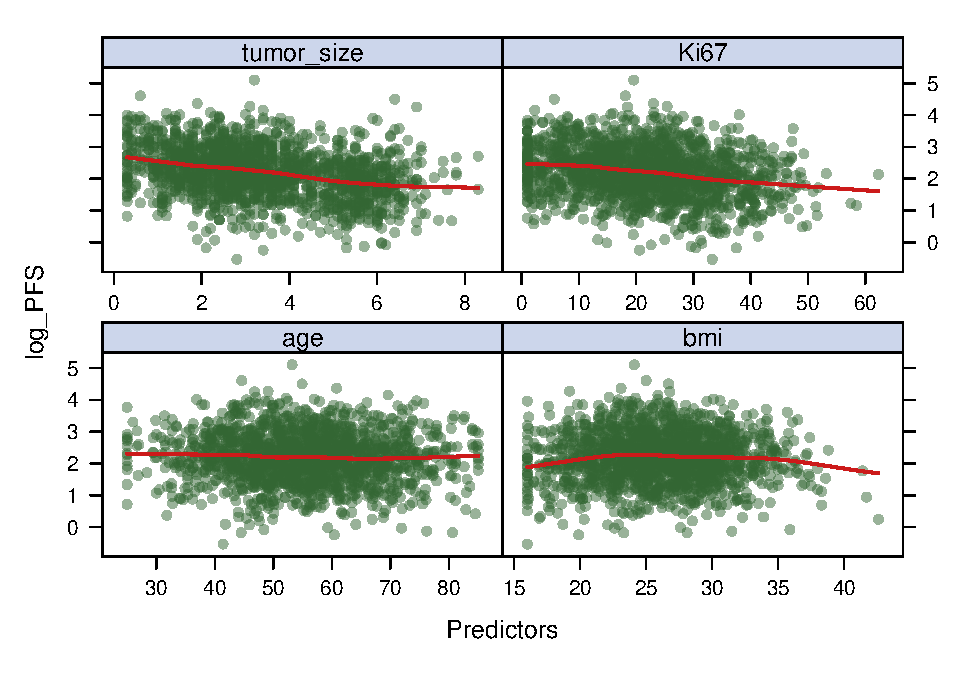
\includegraphics[keepaspectratio]{midterm_files/figure-latex/unnamed-chunk-3-1.pdf}}

\begin{Shaded}
\begin{Highlighting}[]
\CommentTok{\# Calculates the correlation matrix for all the predictors}
\FunctionTok{corrplot}\NormalTok{(}\FunctionTok{cor}\NormalTok{(x\_trainA), }\AttributeTok{method =} \StringTok{"circle"}\NormalTok{, }\AttributeTok{type =} \StringTok{"full"}\NormalTok{)}
\end{Highlighting}
\end{Shaded}

\pandocbounded{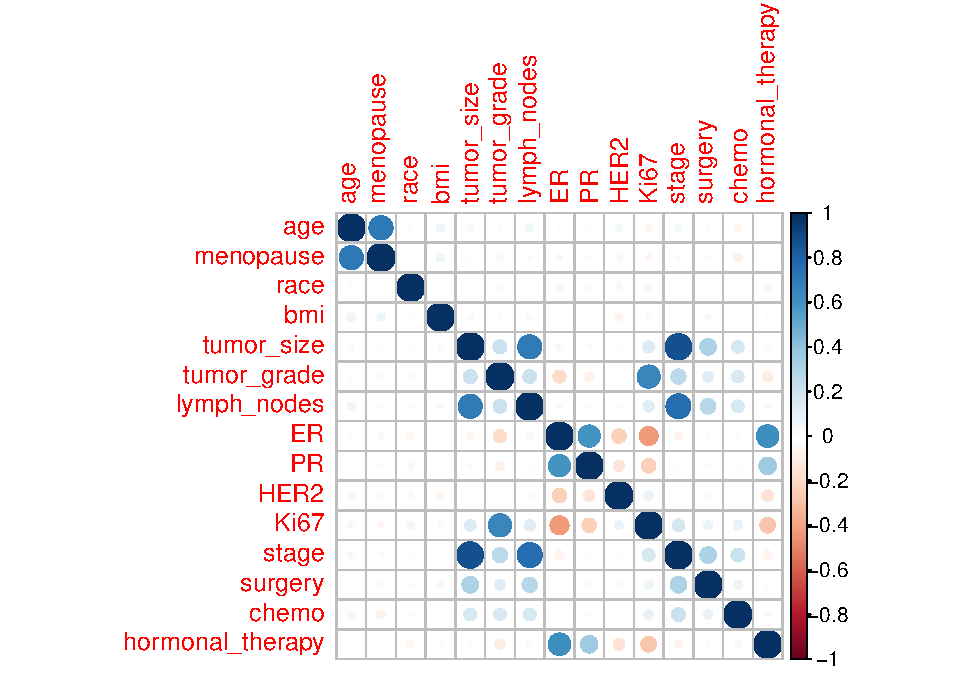
\includegraphics[keepaspectratio]{midterm_files/figure-latex/unnamed-chunk-3-2.pdf}}

This data set includes 7 binary predictors, 3 categorical predictors, 5
continuous predictors, and 1 continuous outcome in log scale.

Chose elastic net because continuous variables formed a cloud, meaning
we could assume linearity? homoscedasticity?

Correlation plot revealed that certain variables were highly correlated.
Chose to address this with elastic net because we can address
colinearity for {[}{]} and {[}{]} reasons

\begin{Shaded}
\begin{Highlighting}[]
\CommentTok{\# Elastic Net}

\NormalTok{ctrl1 }\OtherTok{\textless{}{-}} \FunctionTok{trainControl}\NormalTok{(}\AttributeTok{method =} \StringTok{"cv"}\NormalTok{, }\AttributeTok{number =} \DecValTok{10}\NormalTok{) }\CommentTok{\# set up cv}
\FunctionTok{set.seed}\NormalTok{(}\DecValTok{2}\NormalTok{) }\CommentTok{\# set seed for reproduction}

\CommentTok{\# remove ID}
\NormalTok{training\_datA }\OtherTok{\textless{}{-}}\NormalTok{ training\_datA }\SpecialCharTok{|\textgreater{}}  \FunctionTok{select}\NormalTok{(}\SpecialCharTok{{-}}\StringTok{"id"}\NormalTok{)}
\NormalTok{testing\_datA  }\OtherTok{\textless{}{-}}\NormalTok{ testing\_datA  }\SpecialCharTok{|\textgreater{}} \FunctionTok{select}\NormalTok{(}\SpecialCharTok{{-}}\StringTok{"id"}\NormalTok{)}

\NormalTok{enet.fit }\OtherTok{\textless{}{-}} \FunctionTok{train}\NormalTok{(log\_PFS }\SpecialCharTok{\textasciitilde{}}\NormalTok{ ., }
                  \AttributeTok{data =}\NormalTok{ training\_datA, }
                  \AttributeTok{method =} \StringTok{"glmnet"}\NormalTok{,}
                  \AttributeTok{tuneGrid =} \FunctionTok{expand.grid}\NormalTok{(}\AttributeTok{alpha =} \FunctionTok{seq}\NormalTok{(}\DecValTok{0}\NormalTok{, }\DecValTok{1}\NormalTok{, }\AttributeTok{length =} \DecValTok{21}\NormalTok{),}
                                         \AttributeTok{lambda =} \FunctionTok{exp}\NormalTok{(}\FunctionTok{seq}\NormalTok{(}\SpecialCharTok{{-}}\DecValTok{1}\NormalTok{, }\SpecialCharTok{{-}}\DecValTok{7}\NormalTok{, }\AttributeTok{length =} \DecValTok{100}\NormalTok{))),}
                  \AttributeTok{trControl =}\NormalTok{ ctrl1)}
\end{Highlighting}
\end{Shaded}

\begin{verbatim}
## Warning in nominalTrainWorkflow(x = x, y = y, wts = weights, info = trainInfo,
## : There were missing values in resampled performance measures.
\end{verbatim}

\begin{Shaded}
\begin{Highlighting}[]
\NormalTok{enet.fit}\SpecialCharTok{$}\NormalTok{bestTune}
\end{Highlighting}
\end{Shaded}

\begin{verbatim}
##      alpha     lambda
## 1944  0.95 0.01235197
\end{verbatim}

\begin{Shaded}
\begin{Highlighting}[]
\NormalTok{myCol }\OtherTok{\textless{}{-}} \FunctionTok{rainbow}\NormalTok{(}\DecValTok{25}\NormalTok{)}
\NormalTok{myPar }\OtherTok{\textless{}{-}} \FunctionTok{list}\NormalTok{(}\AttributeTok{superpose.symbol =} \FunctionTok{list}\NormalTok{(}\AttributeTok{col =}\NormalTok{ myCol),}
\AttributeTok{superpose.line =} \FunctionTok{list}\NormalTok{(}\AttributeTok{col =}\NormalTok{ myCol))}

\FunctionTok{plot}\NormalTok{(enet.fit, }\AttributeTok{par.settings =}\NormalTok{ myPar, }\AttributeTok{xTrans =}\NormalTok{ log)}
\end{Highlighting}
\end{Shaded}

\pandocbounded{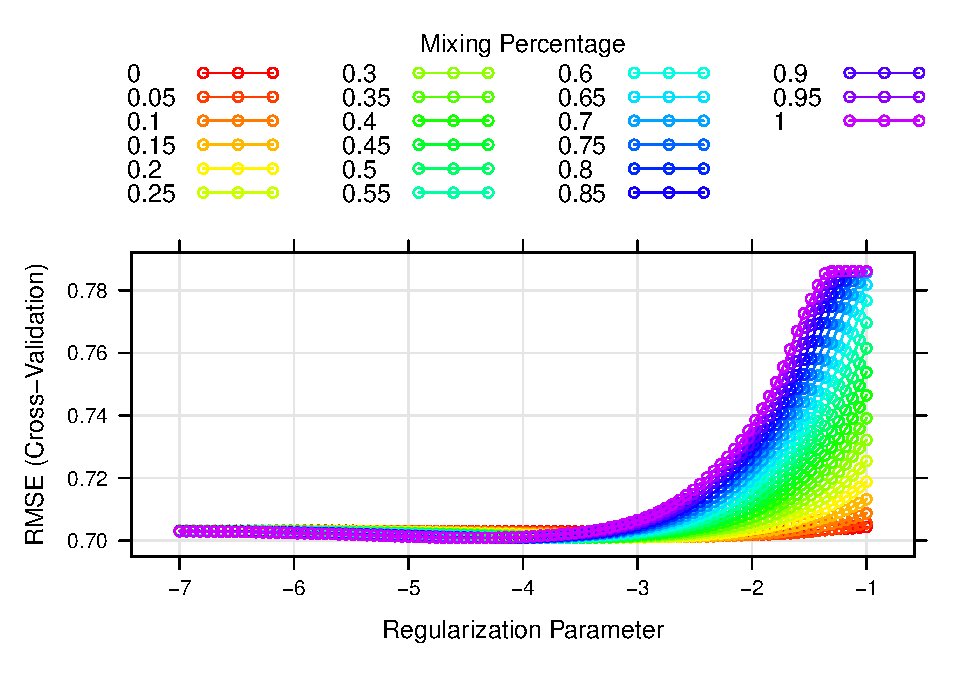
\includegraphics[keepaspectratio]{midterm_files/figure-latex/unnamed-chunk-4-1.pdf}}

\begin{Shaded}
\begin{Highlighting}[]
\CommentTok{\# coefficients in the final model}
\FunctionTok{coef}\NormalTok{(enet.fit}\SpecialCharTok{$}\NormalTok{finalModel, enet.fit}\SpecialCharTok{$}\NormalTok{bestTune}\SpecialCharTok{$}\NormalTok{lambda)}
\end{Highlighting}
\end{Shaded}

\begin{verbatim}
## 16 x 1 sparse Matrix of class "dgCMatrix"
##                  s=0.01235197
## (Intercept)       2.656050011
## age              -0.001046560
## menopause         .          
## race              .          
## bmi               .          
## tumor_size       -0.057703954
## tumor_grade      -0.066041243
## lymph_nodes      -0.056993530
## ER                0.220684085
## PR                .          
## HER2             -0.176250264
## Ki67             -0.003932773
## stage             .          
## surgery           .          
## chemo             .          
## hormonal_therapy  0.137999051
\end{verbatim}

Still to do: predict on testing\_datA

\begin{Shaded}
\begin{Highlighting}[]
\CommentTok{\# predict on testing\_datA}
\NormalTok{enet.pred }\OtherTok{\textless{}{-}} \FunctionTok{predict}\NormalTok{(enet.fit, }\AttributeTok{newdata =}\NormalTok{ testing\_datA)}

\CommentTok{\# test error (MSE)}
\FunctionTok{mean}\NormalTok{((enet.pred }\SpecialCharTok{{-}}\NormalTok{ testing\_datA[, }\StringTok{"log\_PFS"}\NormalTok{])}\SpecialCharTok{\^{}}\DecValTok{2}\NormalTok{)}
\end{Highlighting}
\end{Shaded}

\begin{verbatim}
## [1] 0.4955286
\end{verbatim}

Results: Report the model. Interpret the model and assess its
performance.

\begin{Shaded}
\begin{Highlighting}[]
\CommentTok{\# Create a table with the model coefficients}
\NormalTok{coefs1 }\OtherTok{\textless{}{-}} \FunctionTok{as.data.frame}\NormalTok{(}\FunctionTok{as.matrix}\NormalTok{(}\FunctionTok{coef}\NormalTok{(enet.fit}\SpecialCharTok{$}\NormalTok{finalModel, enet.fit}\SpecialCharTok{$}\NormalTok{bestTune}\SpecialCharTok{$}\NormalTok{lambda)))}
\NormalTok{coefs1}\SpecialCharTok{$}\NormalTok{Predictors }\OtherTok{\textless{}{-}} \FunctionTok{rownames}\NormalTok{(coefs1)}
\FunctionTok{colnames}\NormalTok{(coefs1)[}\DecValTok{1}\NormalTok{] }\OtherTok{\textless{}{-}} \StringTok{"Coefficients"}
\NormalTok{coefs1 }\OtherTok{\textless{}{-}}\NormalTok{ coefs1[, }\FunctionTok{c}\NormalTok{(}\StringTok{"Predictors"}\NormalTok{, }\StringTok{"Coefficients"}\NormalTok{)]}
\FunctionTok{rownames}\NormalTok{(coefs1) }\OtherTok{\textless{}{-}} \ConstantTok{NULL}
\NormalTok{coefs1 }\SpecialCharTok{|\textgreater{}}
  \FunctionTok{kable}\NormalTok{()}
\end{Highlighting}
\end{Shaded}

\begin{longtable}[]{@{}lr@{}}
\toprule\noalign{}
Predictors & Coefficients \\
\midrule\noalign{}
\endhead
\bottomrule\noalign{}
\endlastfoot
(Intercept) & 2.6560500 \\
age & -0.0010466 \\
menopause & 0.0000000 \\
race & 0.0000000 \\
bmi & 0.0000000 \\
tumor\_size & -0.0577040 \\
tumor\_grade & -0.0660412 \\
lymph\_nodes & -0.0569935 \\
ER & 0.2206841 \\
PR & 0.0000000 \\
HER2 & -0.1762503 \\
Ki67 & -0.0039328 \\
stage & 0.0000000 \\
surgery & 0.0000000 \\
chemo & 0.0000000 \\
hormonal\_therapy & 0.1379991 \\
\end{longtable}

\begin{Shaded}
\begin{Highlighting}[]
\CommentTok{\# Create a table with the model coefficients exponentiated}
\NormalTok{coefs2 }\OtherTok{\textless{}{-}} \FunctionTok{as.data.frame}\NormalTok{(}\FunctionTok{as.matrix}\NormalTok{(}\FunctionTok{coef}\NormalTok{(enet.fit}\SpecialCharTok{$}\NormalTok{finalModel, enet.fit}\SpecialCharTok{$}\NormalTok{bestTune}\SpecialCharTok{$}\NormalTok{lambda)))}
\NormalTok{coefs2}\SpecialCharTok{$}\NormalTok{Predictors }\OtherTok{\textless{}{-}} \FunctionTok{rownames}\NormalTok{(coefs2)}
\FunctionTok{colnames}\NormalTok{(coefs2)[}\DecValTok{1}\NormalTok{] }\OtherTok{\textless{}{-}} \StringTok{"Exponentiated Coefficients"}
\NormalTok{coefs2 }\OtherTok{\textless{}{-}}\NormalTok{ coefs2[, }\FunctionTok{c}\NormalTok{(}\StringTok{"Predictors"}\NormalTok{, }\StringTok{"Exponentiated Coefficients"}\NormalTok{)]}
\NormalTok{coefs2 }\OtherTok{\textless{}{-}}\NormalTok{ coefs2 }\SpecialCharTok{|\textgreater{}}
  \FunctionTok{filter}\NormalTok{(Predictors }\SpecialCharTok{\%in\%} \FunctionTok{c}\NormalTok{(}\StringTok{"(Intercept)"}\NormalTok{, }\StringTok{"age"}\NormalTok{, }\StringTok{"tumor\_size"}\NormalTok{, }\StringTok{"tumor\_grade"}\NormalTok{, }\StringTok{"lymph\_nodes"}\NormalTok{, }
                           \StringTok{"ER"}\NormalTok{, }\StringTok{"HER2"}\NormalTok{, }\StringTok{"Ki67"}\NormalTok{, }\StringTok{"hormonal\_therapy"}\NormalTok{))}
\NormalTok{coefs2}\SpecialCharTok{$}\StringTok{\textasciigrave{}}\AttributeTok{Exponentiated Coefficients}\StringTok{\textasciigrave{}}\OtherTok{\textless{}{-}} \FunctionTok{exp}\NormalTok{(coefs2}\SpecialCharTok{$}\StringTok{\textasciigrave{}}\AttributeTok{Exponentiated Coefficients}\StringTok{\textasciigrave{}}\NormalTok{)}
\FunctionTok{rownames}\NormalTok{(coefs2) }\OtherTok{\textless{}{-}} \ConstantTok{NULL}
\NormalTok{coefs2 }\SpecialCharTok{|\textgreater{}}
  \FunctionTok{kable}\NormalTok{()}
\end{Highlighting}
\end{Shaded}

\begin{longtable}[]{@{}lr@{}}
\toprule\noalign{}
Predictors & Exponentiated Coefficients \\
\midrule\noalign{}
\endhead
\bottomrule\noalign{}
\endlastfoot
(Intercept) & 14.2399303 \\
age & 0.9989540 \\
tumor\_size & 0.9439294 \\
tumor\_grade & 0.9360923 \\
lymph\_nodes & 0.9446002 \\
ER & 1.2469294 \\
HER2 & 0.8384081 \\
Ki67 & 0.9960750 \\
hormonal\_therapy & 1.1479745 \\
\end{longtable}

\section{Part II}\label{part-ii}

About a decade later, Researcher B conducted a separate study enrolling
2000 breast cancer patients diagnosed between 2000 and 2005, using the
same study design and variable definitions. Like Researcher A's study,
all patients were followed until disease progression or death.
Researcher B's data are stored in datB.RData. Researcher A would like to
evaluate whether the prediction model built on the original data
generalizes well to Researcher B's dataset. Does the model generalize
well? If yes, provide justification. If not, build a new prediction
model for the 2000--2005 cohort and discuss what has changed in
prediction.

\subsection{Import and explore the full
dataset}\label{import-and-explore-the-full-dataset}

\begin{Shaded}
\begin{Highlighting}[]
\FunctionTok{load}\NormalTok{(}\StringTok{"data/datB.RData"}\NormalTok{)}

\CommentTok{\# basic summary}
\FunctionTok{summary}\NormalTok{(datB)}
\end{Highlighting}
\end{Shaded}

\begin{verbatim}
##       id                 age          menopause          race      
##  Length:2000        Min.   :25.00   Min.   :0.000   Min.   :1.000  
##  Class :character   1st Qu.:48.50   1st Qu.:0.000   1st Qu.:1.000  
##  Mode  :character   Median :56.00   Median :1.000   Median :1.000  
##                     Mean   :56.05   Mean   :0.681   Mean   :1.875  
##                     3rd Qu.:63.80   3rd Qu.:1.000   3rd Qu.:3.000  
##                     Max.   :85.00   Max.   :1.000   Max.   :4.000  
##       bmi          tumor_size     tumor_grade     lymph_nodes    
##  Min.   :16.00   Min.   :0.300   Min.   :1.000   Min.   : 0.000  
##  1st Qu.:24.00   1st Qu.:1.800   1st Qu.:1.000   1st Qu.: 0.000  
##  Median :27.30   Median :2.800   Median :2.000   Median : 2.000  
##  Mean   :27.44   Mean   :3.075   Mean   :2.079   Mean   : 2.318  
##  3rd Qu.:30.82   3rd Qu.:4.200   3rd Qu.:3.000   3rd Qu.: 4.000  
##  Max.   :45.90   Max.   :7.900   Max.   :3.000   Max.   :15.000  
##        ER              PR              HER2            Ki67      
##  Min.   :0.000   Min.   :0.0000   Min.   :0.000   Min.   : 1.00  
##  1st Qu.:0.000   1st Qu.:0.0000   1st Qu.:0.000   1st Qu.:11.70  
##  Median :1.000   Median :1.0000   Median :0.000   Median :19.85  
##  Mean   :0.674   Mean   :0.5045   Mean   :0.237   Mean   :20.37  
##  3rd Qu.:1.000   3rd Qu.:1.0000   3rd Qu.:0.000   3rd Qu.:28.80  
##  Max.   :1.000   Max.   :1.0000   Max.   :1.000   Max.   :62.30  
##      stage          surgery           chemo       hormonal_therapy
##  Min.   :1.000   Min.   :0.0000   Min.   :0.000   Min.   :0.0000  
##  1st Qu.:1.000   1st Qu.:0.0000   1st Qu.:0.000   1st Qu.:0.0000  
##  Median :2.000   Median :0.0000   Median :1.000   Median :1.0000  
##  Mean   :1.894   Mean   :0.4415   Mean   :0.649   Mean   :0.5695  
##  3rd Qu.:2.000   3rd Qu.:1.0000   3rd Qu.:1.000   3rd Qu.:1.0000  
##  Max.   :3.000   Max.   :1.0000   Max.   :1.000   Max.   :1.0000  
##     log_PFS       
##  Min.   :-0.0866  
##  1st Qu.: 2.2536  
##  Median : 2.7440  
##  Mean   : 2.7424  
##  3rd Qu.: 3.2487  
##  Max.   : 5.2864
\end{verbatim}

\begin{Shaded}
\begin{Highlighting}[]
\CommentTok{\# compare distributions of key variables between datasets}
\FunctionTok{par}\NormalTok{(}\AttributeTok{mfrow =} \FunctionTok{c}\NormalTok{(}\DecValTok{1}\NormalTok{, }\DecValTok{2}\NormalTok{))}
\FunctionTok{hist}\NormalTok{(datA}\SpecialCharTok{$}\NormalTok{age, }\AttributeTok{main =} \StringTok{"Age {-} Training"}\NormalTok{, }\AttributeTok{xlab =} \StringTok{"Age"}\NormalTok{)}
\FunctionTok{hist}\NormalTok{(datB}\SpecialCharTok{$}\NormalTok{age, }\AttributeTok{main =} \StringTok{"Age {-} New Data"}\NormalTok{, }\AttributeTok{xlab =} \StringTok{"Age"}\NormalTok{)}
\end{Highlighting}
\end{Shaded}

\pandocbounded{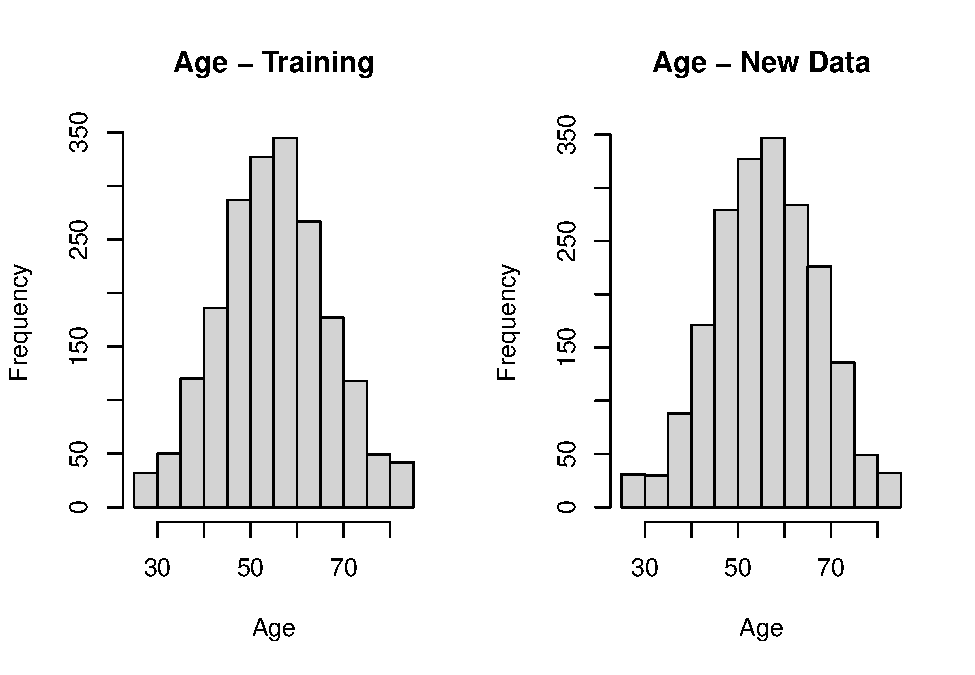
\includegraphics[keepaspectratio]{midterm_files/figure-latex/unnamed-chunk-7-1.pdf}}

\begin{Shaded}
\begin{Highlighting}[]
\FunctionTok{par}\NormalTok{(}\AttributeTok{mfrow =} \FunctionTok{c}\NormalTok{(}\DecValTok{1}\NormalTok{, }\DecValTok{2}\NormalTok{))}
\FunctionTok{hist}\NormalTok{(datA}\SpecialCharTok{$}\NormalTok{tumor\_size, }\AttributeTok{main =} \StringTok{"Tumor Size {-} Training"}\NormalTok{, }\AttributeTok{xlab =} \StringTok{"Tumor Size"}\NormalTok{)}
\FunctionTok{hist}\NormalTok{(datB}\SpecialCharTok{$}\NormalTok{tumor\_size, }\AttributeTok{main =} \StringTok{"Tumor Size {-} New Data"}\NormalTok{, }\AttributeTok{xlab =} \StringTok{"Tumor Size"}\NormalTok{)}
\end{Highlighting}
\end{Shaded}

\pandocbounded{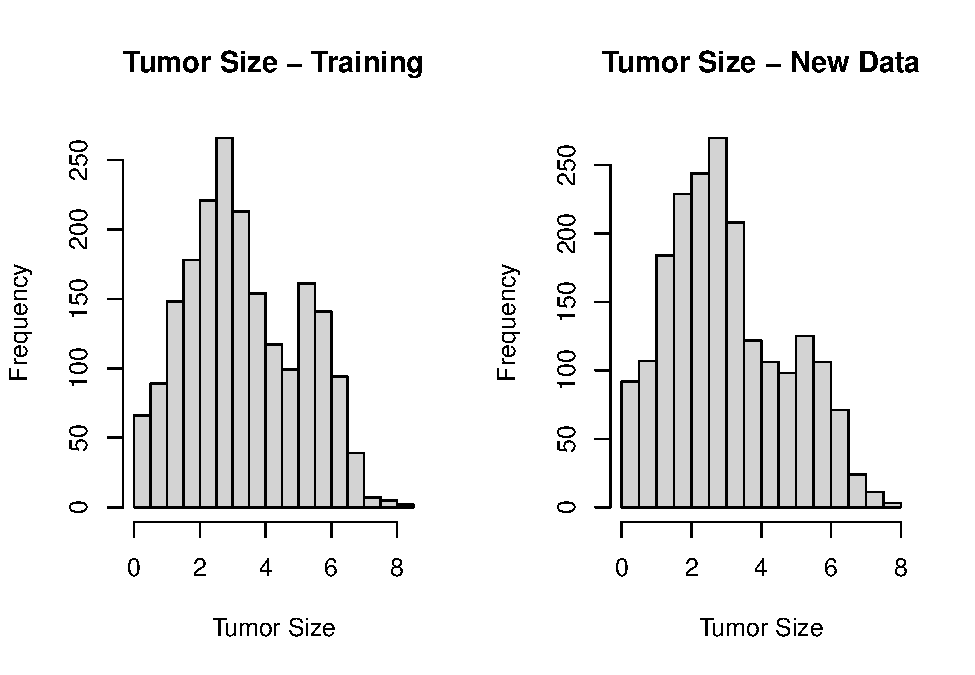
\includegraphics[keepaspectratio]{midterm_files/figure-latex/unnamed-chunk-7-2.pdf}}

\begin{Shaded}
\begin{Highlighting}[]
\FunctionTok{par}\NormalTok{(}\AttributeTok{mfrow =} \FunctionTok{c}\NormalTok{(}\DecValTok{1}\NormalTok{, }\DecValTok{2}\NormalTok{))}
\FunctionTok{hist}\NormalTok{(datA}\SpecialCharTok{$}\NormalTok{tumor\_grade, }\AttributeTok{main =} \StringTok{"Tumor Grade {-} Training"}\NormalTok{, }\AttributeTok{xlab =} \StringTok{"Tumor Grade"}\NormalTok{)}
\FunctionTok{hist}\NormalTok{(datB}\SpecialCharTok{$}\NormalTok{tumor\_grade, }\AttributeTok{main =} \StringTok{"Tumor Grade {-} New Data"}\NormalTok{, }\AttributeTok{xlab =} \StringTok{"Tumor Grade"}\NormalTok{)}
\end{Highlighting}
\end{Shaded}

\pandocbounded{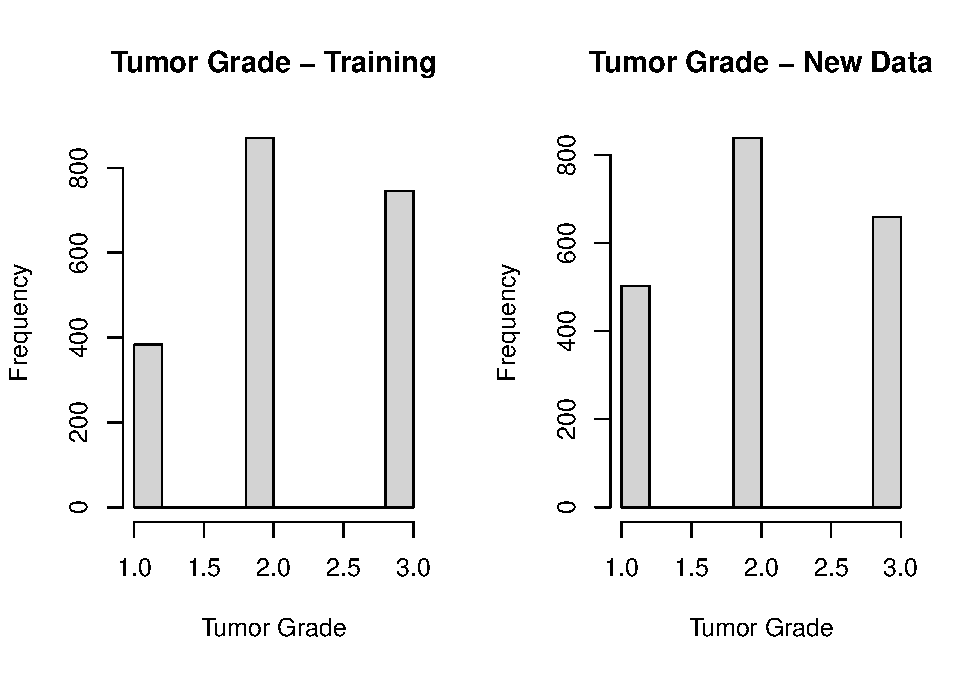
\includegraphics[keepaspectratio]{midterm_files/figure-latex/unnamed-chunk-7-3.pdf}}

\begin{Shaded}
\begin{Highlighting}[]
\CommentTok{\# remove id for matrix operations}
\NormalTok{datB\_clean\_eda }\OtherTok{\textless{}{-}}\NormalTok{ datB }\SpecialCharTok{|\textgreater{}} \FunctionTok{select}\NormalTok{(}\SpecialCharTok{{-}}\StringTok{"id"}\NormalTok{)}
\NormalTok{x\_B\_all }\OtherTok{\textless{}{-}} \FunctionTok{model.matrix}\NormalTok{(log\_PFS }\SpecialCharTok{\textasciitilde{}}\NormalTok{ ., datB\_clean\_eda)[, }\SpecialCharTok{{-}}\DecValTok{1}\NormalTok{]}
\end{Highlighting}
\end{Shaded}

\subsection{Evaluate the model's performance on researcher B's
dataset}\label{evaluate-the-models-performance-on-researcher-bs-dataset}

\begin{Shaded}
\begin{Highlighting}[]
\CommentTok{\# remove ID}
\NormalTok{datB }\OtherTok{\textless{}{-}}\NormalTok{ datB }\SpecialCharTok{|\textgreater{}}  \FunctionTok{select}\NormalTok{(}\SpecialCharTok{{-}}\StringTok{"id"}\NormalTok{)}

\CommentTok{\# use all of datB to test generalizability of elastic net model}
\NormalTok{enet\_pred\_B }\OtherTok{\textless{}{-}} \FunctionTok{predict}\NormalTok{(enet.fit, }\AttributeTok{newdata =}\NormalTok{ datB)}

\CommentTok{\# compare performance (will update once model is tested on datA testing split)}
\CommentTok{\# rmse\_A \textless{}{-} RMSE(enet\_pred\_A,     testing\_datA$log\_PFS)}
\CommentTok{\# r2\_A   \textless{}{-} R2(enet\_pred\_A,       testing\_datA$log\_PFS)}
\NormalTok{rmse\_B }\OtherTok{\textless{}{-}} \FunctionTok{RMSE}\NormalTok{(enet\_pred\_B, datB}\SpecialCharTok{$}\NormalTok{log\_PFS)}
\NormalTok{r2\_B   }\OtherTok{\textless{}{-}} \FunctionTok{R2}\NormalTok{(enet\_pred\_B,   datB}\SpecialCharTok{$}\NormalTok{log\_PFS)}

\CommentTok{\# cat("datA Test RMSE:", round(rmse\_A, 4), "\textbackslash{}n")}
\CommentTok{\# cat("datA Test R²:  ", round(r2\_A,   4), "\textbackslash{}n\textbackslash{}n")}
\FunctionTok{cat}\NormalTok{(}\StringTok{"datB RMSE:     "}\NormalTok{, }\FunctionTok{round}\NormalTok{(rmse\_B, }\DecValTok{4}\NormalTok{), }\StringTok{"}\SpecialCharTok{\textbackslash{}n}\StringTok{"}\NormalTok{)}
\end{Highlighting}
\end{Shaded}

\begin{verbatim}
## datB RMSE:      0.8383
\end{verbatim}

\begin{Shaded}
\begin{Highlighting}[]
\FunctionTok{cat}\NormalTok{(}\StringTok{"datB R²:       "}\NormalTok{, }\FunctionTok{round}\NormalTok{(r2\_B,   }\DecValTok{4}\NormalTok{), }\StringTok{"}\SpecialCharTok{\textbackslash{}n}\StringTok{"}\NormalTok{)}
\end{Highlighting}
\end{Shaded}

\begin{verbatim}
## datB R²:        0.1489
\end{verbatim}

\begin{Shaded}
\begin{Highlighting}[]
\CommentTok{\# will add adjusted r\^{}2}
\end{Highlighting}
\end{Shaded}

The elastic net model explained approximately 15\% of the variance in
the log-transformed PFS in the 2000 to 2005 study cohort, suggesting
weak predictive performance.

\subsection{TO DO ONLY IF NEED TO CREATE NEW
MODEL}\label{to-do-only-if-need-to-create-new-model}

\subsection{Import and partition data using `tidymodels'
package}\label{import-and-partition-data-using-tidymodels-package-1}

\begin{Shaded}
\begin{Highlighting}[]
\FunctionTok{set.seed}\NormalTok{(}\DecValTok{2}\NormalTok{)}

\NormalTok{datB\_split }\OtherTok{=} \FunctionTok{initial\_split}\NormalTok{(datB, }\AttributeTok{prop =} \FloatTok{0.8}\NormalTok{)}

\CommentTok{\#extract the training and test data}
\NormalTok{training\_datB }\OtherTok{=} \FunctionTok{training}\NormalTok{(datB\_split)}
\NormalTok{testing\_datB }\OtherTok{=} \FunctionTok{testing}\NormalTok{(datB\_split)}

\CommentTok{\#training data}
\NormalTok{x\_trainB }\OtherTok{=} \FunctionTok{model.matrix}\NormalTok{(log\_PFS }\SpecialCharTok{\textasciitilde{}}\NormalTok{ ., training\_datB)[, }\SpecialCharTok{{-}}\DecValTok{1}\NormalTok{]}
\NormalTok{y\_trainB }\OtherTok{=}\NormalTok{ training\_datB}\SpecialCharTok{$}\NormalTok{log\_PFS}

\CommentTok{\#test data}
\NormalTok{x\_testB  }\OtherTok{=} \FunctionTok{model.matrix}\NormalTok{(log\_PFS }\SpecialCharTok{\textasciitilde{}}\NormalTok{ ., testing\_datB)[, }\SpecialCharTok{{-}}\DecValTok{1}\NormalTok{]}
\NormalTok{y\_testB }\OtherTok{=}\NormalTok{ testing\_datB}\SpecialCharTok{$}\NormalTok{log\_PFS}
\end{Highlighting}
\end{Shaded}

\subsection{Exploratory Data
Analysis}\label{exploratory-data-analysis-1}

\begin{Shaded}
\begin{Highlighting}[]
\CommentTok{\# Feature plots to look at trends between predictors and the outcome (log\_PFS)}
\CommentTok{\# featurePlot(x = training\_datB[ ,2:16],}
\CommentTok{\#             y = training\_datB[ ,17],}
\CommentTok{\#             plot = "scatter",}
\CommentTok{\#             span = .5,}
\CommentTok{\#             labels = c("Predictors","log\_PFS"),}
\CommentTok{\#             type = c("p", "smooth"),}
\CommentTok{\#             layout = c(3, 2))}
\CommentTok{\# }
\CommentTok{\# \# Calculates the correlation matrix for all the predictors}
\CommentTok{\# corrplot(cor(x\_trainB), method = "circle", type = "full")}
\end{Highlighting}
\end{Shaded}

\section{GAM model}\label{gam-model}

\begin{Shaded}
\begin{Highlighting}[]
\NormalTok{mars.fit }\OtherTok{\textless{}{-}} \FunctionTok{train}\NormalTok{(log\_PFS }\SpecialCharTok{\textasciitilde{}}\NormalTok{ .,}
                  \AttributeTok{data =}\NormalTok{ training\_datA,}
                  \AttributeTok{method =} \StringTok{"earth"}\NormalTok{,}
                  \AttributeTok{tuneGrid =} \FunctionTok{expand.grid}\NormalTok{(}\AttributeTok{degree =} \DecValTok{1}\SpecialCharTok{:}\DecValTok{3}\NormalTok{,}
                                        \AttributeTok{nprune =} \DecValTok{2}\SpecialCharTok{:}\DecValTok{20}\NormalTok{),}
                  \AttributeTok{trControl =}\NormalTok{ ctrl1)}

\NormalTok{mars.fit}\SpecialCharTok{$}\NormalTok{bestTune}
\end{Highlighting}
\end{Shaded}

\begin{verbatim}
##   nprune degree
## 9     10      1
\end{verbatim}

\begin{Shaded}
\begin{Highlighting}[]
\CommentTok{\# evaluate on testing\_datA (internal test split)}
\NormalTok{pred\_mars\_testA }\OtherTok{\textless{}{-}} \FunctionTok{predict}\NormalTok{(mars.fit, }\AttributeTok{newdata =}\NormalTok{ testing\_datA)}
\NormalTok{rmse\_mars\_testA }\OtherTok{\textless{}{-}} \FunctionTok{sqrt}\NormalTok{(}\FunctionTok{mean}\NormalTok{((pred\_mars\_testA }\SpecialCharTok{{-}}\NormalTok{ testing\_datA}\SpecialCharTok{$}\NormalTok{log\_PFS)}\SpecialCharTok{\^{}}\DecValTok{2}\NormalTok{))}
\NormalTok{r2\_mars\_testA }\OtherTok{\textless{}{-}} \FunctionTok{cor}\NormalTok{(pred\_mars\_testA, testing\_datA}\SpecialCharTok{$}\NormalTok{log\_PFS)}\SpecialCharTok{\^{}}\DecValTok{2}

\CommentTok{\# evaluate on datB (external validation)}
\NormalTok{pred\_mars\_B }\OtherTok{\textless{}{-}} \FunctionTok{predict}\NormalTok{(mars.fit, }\AttributeTok{newdata =}\NormalTok{ datB)}
\NormalTok{rmse\_mars\_B }\OtherTok{\textless{}{-}} \FunctionTok{sqrt}\NormalTok{(}\FunctionTok{mean}\NormalTok{((pred\_mars\_B }\SpecialCharTok{{-}}\NormalTok{ datB}\SpecialCharTok{$}\NormalTok{log\_PFS)}\SpecialCharTok{\^{}}\DecValTok{2}\NormalTok{))}
\NormalTok{r2\_mars\_B }\OtherTok{\textless{}{-}} \FunctionTok{cor}\NormalTok{(pred\_mars\_B, datB}\SpecialCharTok{$}\NormalTok{log\_PFS)}\SpecialCharTok{\^{}}\DecValTok{2}
\end{Highlighting}
\end{Shaded}

Run GAM or MARs if model isn't super generalizable?

\end{document}
